\section{Testszenarien} %
In diesem Abschnitt werden die Testszenarien beschrieben, wie die einzelnen Hardwarekomponenten ESP32 und FPGA und die Verbindungstest zwischen den Komponenten gestestet wurde.

\subsection{ESP32 SPI und Statemachine Test}
\label{sub:ESPSPIundFSMTest}

Für die Verifikation der Firmware auf dem ESP32-S3 wurde ein zweites Gerät, welches als SPI-Master den FPGA simulieren soll, verwendet. Die Hardware, welche als SPI Master verwendet wurde war ein ESP32. Dies aus dem Grund, weil bereits Erfahrungen mit dem ESP32 vorhanden waren und ein Aufsetzten des Gerätes und Ausgeben schnell erreicht wurde. In Abbildung \ref{fig:TestszenarioESP32} ist der schematische Aufbau zu sehen. Es wurden die Verbindungen für die SPI-Leitungen und GND verbunden. Auf einem Laptop wurde die Open-Source-Software Bluetility verwendet, ein Bluetooth-Low-Energy-Tool. Mit dieser Anwendung können Geräte gescannt, deren Dienste und Eigenschaften durchsucht sowie Werte gelesen, geschrieben und abonniert werden. Gemäss Kapitel \ref{sub:BluetoothGATT} wurden die Daten in der Charakteristik mit der roten Zahl 1 empfangen. Zusätzlich wird die Reaktionszeit beim Empfangen der SPI-Daten gemessen. Dies wird durch das Vergleichen der Chip Select-Leitung und der Handshakeleitung. 

\begin{figure}[H]
    \centering
    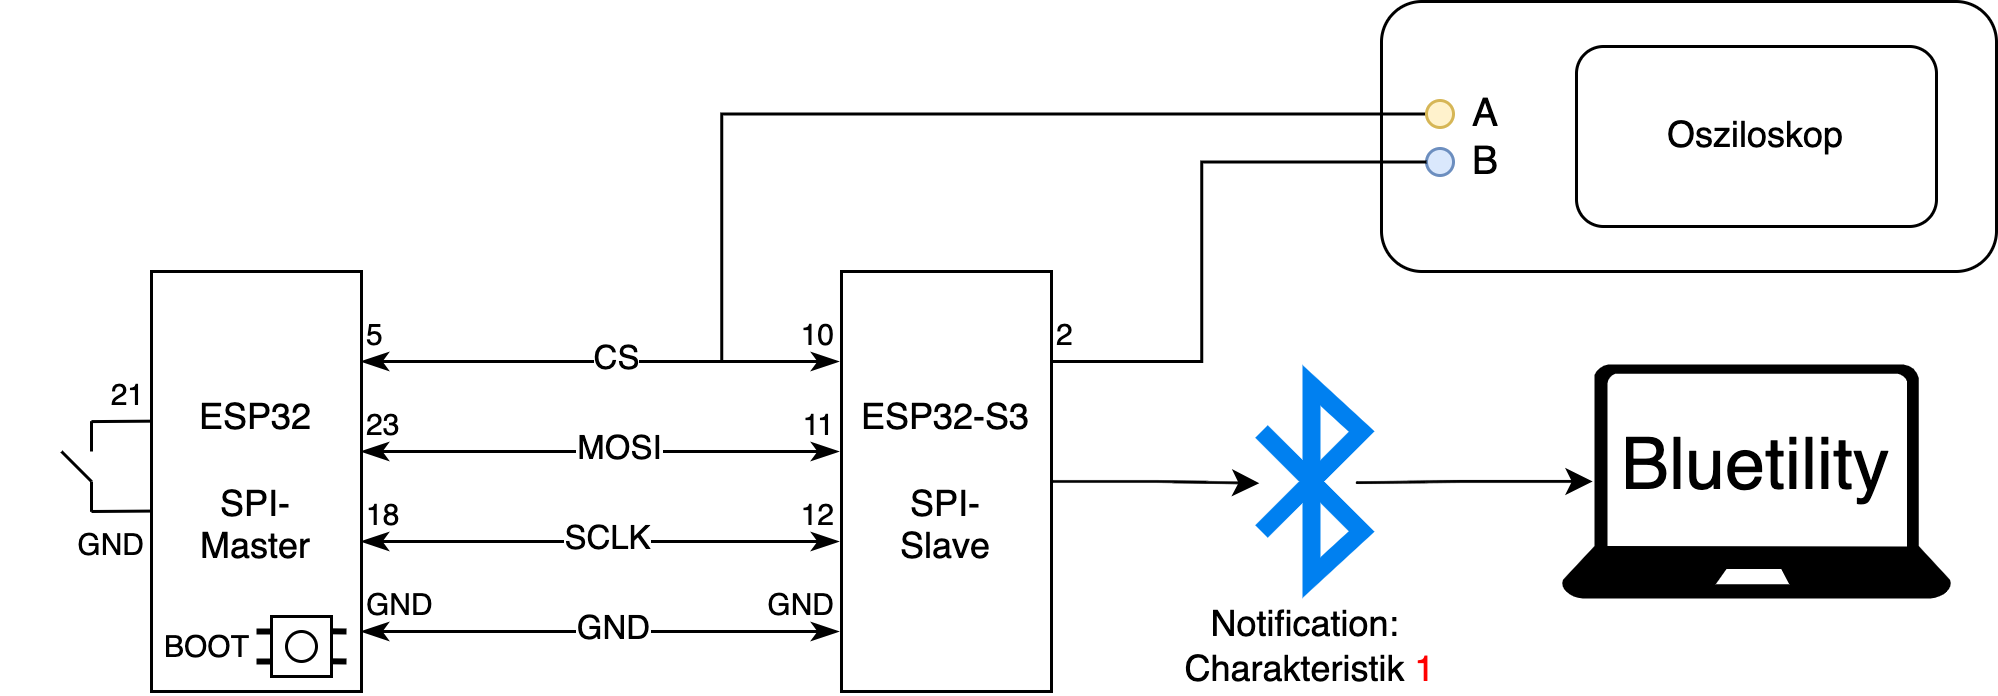
\includegraphics[width=0.9\linewidth]{Figures/Chap3/Testszenarien/Testszenario_ESP32.png}
    \caption{Testaufbau zum Testen der Manchester Decodierung auf dem ESP32-S3}
    \label{fig:TestszenarioESP32}
\end{figure}

Der SPI-Master konnte zwei unterschiedliche Telegramme schicken. Es kann entweder das kürzeste oder das längste Telegramm geschickt werden. Die Auswahl ist von Pin 21 (siehe Abbildung \ref{fig:TestszenarioESP32}) abhängig. Wird dieser Pin zu Ground gezogen, wird das lange Telegramm geschickt und wird der Kontakt offen gelassen, das Kurze. Das Senden eines Paketes wird durch Drücken des Boot-Knopfes ausgelöst. Dies zieht den Pin 0 zu Ground und das kann im Programm ausgewertet werden. 

Der Inhalt, der in Tabelle \ref{tab:TestDataESP32} zu sehen ist, sind die Nutzdatenbits, welche bei Bluetility ankommen sollen. Der SPI-Master schickt die Daten wie der FPGA Machnester Encodiert in 64 Bit-Päckchen, also jeweils 32 Bit Nutzdatenbits. Bei den Slave Daten wurde absichtlich ein lesbarer ASCII String für die Dummy Daten verwendet, da diese in Bluetility gleich ersichtlich ist.

\begin{table}[H]
    \centering
    \begin{tabular}{r||l|l}
         & Kurz & Lang\\ \hline
        FCode & 9 (0x9) & 12 (0xC)\\ \hline
        Addresse & 0x101 & 0x0D8\\ \hline
        Master Check & 0xF0 & 0x21\\ \hline
        Slave Data & NH & Hello World 01234567890123456789\\ \hline
        Slave Check & 0x53 & 0x5A 0x98 0x70 0x5d\\ 
    \end{tabular}
    \caption{Test Daten für Testszenario ESP32}
    \label{tab:TestDataESP32}
\end{table}




\subsection{Verbindungstest ESP32 zu FPGA}
\textcolor{red}{Wie wurde der Aufbau getestet}

Um zu testen ob die Decodierung des Manchestersignal bis hin zur Übertragung via Bluetooth korrekt funktioniert, wurde ein Testaufbau realisiert. Für den Aufbau wurden die verschiedenen Komponenten des Sniffers wie in Abbildung \ref{fig:AufbauSniffer} zu sehen ist, verbunden. Als Signalquelle wurde ein \textcolor{red}{\textit{Tektronix}} verwendet. Mit dem Tektronix ist es möglich über die beiden Outputs A \& B ein differentielles Signal auszugeben. Somit wurde das Signal welches zur Bestimmung der Busauslastung (siehe Kapitel \ref{fig:MessaufbauBusauslastungMessen}) aufgenommen wurde, mittels Matlab und \textcolor{red}{\textit{???Programm???}} so aufbereitet, dass dieses mit dem Tektronix abgespielt werden konnte.
Somit kann genau festgestellt werden ob die übertragenen Daten, dem Signal entsprechen und ob die Daten stabil und Fehlerfrei übertragen werden. Das Signal wurde zur Überprüfung im Vorhinein manuell decodiert.
Zur Prüfung wurden folgende Master und Slave Telegramme übertragen:

\begin{itemize}
  \item \textbf{Master Frame 1:}\hspace{0.5cm}0xC715'569A'6555'99A6\newline\textbf{Slave Frame 1:}\hspace{0.75cm}0xA8E3'5565'9A65'AAAA'AAAA'6A66
  \item \textbf{Master Frame 2:}\hspace{0.5cm}0xC715'5699'5A55'6AAA\newline\textbf{Slave Frame 2:}\hspace{0.75cm}0xA8E3'5565'A996'AAAA'AAAA'A569
  \item \textbf{Master Frame 3:}\hspace{0.5cm}0xC715'9656'5655'6AA9
\end{itemize}

Diese Telegramme entsprechen dem in \textit{Abbildung \ref{fig:AusschnittMvbOhneDds}} zu sehende Signal.

Die oben gezeigte Datenabfolge gibt Schlussendlich per Bluetooth folgenden Payload aus:

\begin{itemize}
  \item \textbf{Master Frame 1:}\hspace{0.5cm}0x1B'40'AD\hspace{1.5cm}\textbf{Slave Frame 1:}\hspace{0.5cm}0x04'B4'FF'FF'75
  \item \textbf{Master Frame 2:}\hspace{0.5cm}0x08'60'EF\hspace{1.7cm}\textbf{Slave Frame 2:}\hspace{0.5cm}0x00'00'FF
  \item \textbf{Master Frame 3:}\hspace{0.5cm}0x91'10'7E
\end{itemize}
